\documentclass[12pt]{article}

% Document Setup
% ==============

\author{Steffen Haug}
%% remove the temporary files (.bcf, .aux, ...) if
%% you change the language, because this invalidates
%% the cached babel settings.
\usepackage[nynorsk]{babel}

\usepackage{csquotes}
\usepackage[style=phys]{biblatex}
\usepackage{scalerel}
\usepackage{relsize}

\usepackage{bm, upgreek}

\usepackage{mathtools} % coloneqq
\usepackage{siunitx}
\usepackage{textcomp}

\usepackage{unicode-math}

% Get mathbb and mathcal back (unicode-math replaces them)
\DeclareMathAlphabet{\mathcal}{OMS}{cmsy}{m}{n}
\let\mathbb\relax % remove the definition by unicode-math
\DeclareMathAlphabet{\mathbb}{U}{msb}{m}{n}

\setmainfont{EB Garamond}
\setmonofont{Courier New}
\setmathfont[StylisticSet={7, 2, 10}]{Garamond-Math}


% Custom Commands
% ---------------
\newcommand{\Vect}[1]{{\mathbf{#1}}}
\let\vec\Vect

\newcommand{\Mat}[1]{\mathbf{\mathrm{#1}}}

\newcommand{\deldel}[2]{\frac{\partial #1}{\partial #2}}
\newcommand{\deldelN}[3]{\frac{\partial^{#3} #1}{\partial #2 ^{#3}}}
\newcommand{\dd}[2]{\frac{\mathrm d #1}{\mathrm d #2}}
\newcommand{\textdd}[2]{{\mathrm d #1}/{\mathrm d #2}}
\newcommand{\Tay}[3]{T_{#2}\left \{ #1 \right \}(#3)}
\newcommand{\LRSeq}[1]{\left\{ #1 \right\}}
\newcommand{\Seq}[1]{\big\{ #1 \big\}}

%% fourier transform
\newcommand{\FT}[2]{
    \frac{1}{\sqrt{2\pi}} \smashoperator{\int\limits_{#1=-\infty\mathstrut}^{#1=\infty\mathstrut}}
        #2 e^{-i\omega #1} \D #1
}

\newcommand{\Err}[1]{\mathrm{error}_{#1}}
\newcommand{\Diam}{\mathrm{diam}}
\newcommand{\D}{\mathrm{d}}

\newcommand{\R}{\mathbb{R}}
\newcommand{\N}{\mathbb{N}}
\newcommand{\C}{\mathbb{C}}

\newcommand{\Norm}[2][]{\left\lVert#2\right\rVert_{#1}}
\newcommand{\Jac}[1][]{\mathbf{J}_{#1}}
\newcommand{\Diag}[1]{\mathrm{diag} #1}


\newcommand{\Fig}[1]{\mbox{\scshape figure \ref{fig:#1}}}
\newcommand{\Tab}[1]{\mbox{\scshape table \ref{table:#1}}}

\DeclareMathOperator*{\Sub}{\Bigg\vert}

% smash bounding boxes. useful for limits etc.
% \def\mathclap#1{\text{\hbox to 0pt{\hss$\mathsurround=0pt#1$\hss}}}

% -- Text Formatting
\linespread{1.10}

% -- Custom Titles
\usepackage{titlesec}

\renewcommand\thesection{\Roman{section}}
\renewcommand\thesubsection{\normalfont\roman{subsection}}
\titleformat{name=\section,numberless}[block]{\Large\scshape}{}{0pt}{}
\titleformat{name=\section}[block]{\Large\scshape}{\thesection.}{5pt}{}

\titleformat{name=\subsection,numberless}[block]{\filcenter\large\scshape}{}{0pt}{}
\titleformat{name=\subsection}[block]{\filcenter\large\scshape}{\thesubsection.}{5pt}{}

\usepackage{moresize}
\usepackage{abstract}
\usepackage{appendix}

\renewcommand{\abstractnamefont}{\normalfont\scshape}
\renewcommand{\abstracttextfont}{\normalfont\small}

% -- Title Section
\usepackage{titling} % Customising the title section
\setlength{\droptitle}{-5\baselineskip} % Move the title up

% Document margins optimized for two-column layout; they
\usepackage[
    marginparwidth=35mm,
    right=15mm,
    left=15mm,
    head=15pt,
]{geometry}
\setlength{\columnsep}{5mm}
\usepackage{afterpage}
\usepackage{pagecolor}

% -- Headers and footers
\usepackage{fancyhdr}
\pagestyle{fancy}
\fancyhead{}
\fancyfoot{}
\fancyfoot[C]{\thepage}


% clean up the "plain" style.
\fancypagestyle{plain}{\
  \fancyhf{}
  \renewcommand{\headrulewidth}{0pt}
}


\usepackage{float}
\usepackage{multicol}
\usepackage{graphics}

% -- Custom captions
\usepackage[hang,small,labelfont=bf,up,textfont=it,up]{caption}

% -- Compact lists
\usepackage{enumitem}
\setlist[itemize]{noitemsep}

% -- LISTINGS --
\usepackage{listings}
% Options for all coding environments
\lstset{
    basicstyle=\scriptsize\ttfamily
}
\lstset{
    frame=tb,
    framexleftmargin=2.5em,
    numbers=left,
    xleftmargin=2.5em,
    showstringspaces=false,
}

% The built-in python highlighter is for python2,
% so we need to modify it:
\newcommand\pythonstyle{\lstset{
language=Python,
morekeywords={self, yield, as, assert, pass},
}}

% python env.
\lstnewenvironment{python}[1][]
{
\pythonstyle
\lstset{#1}
}
{}

% inline pytohn env.
\newcommand\pythoninline[1]{{\pythonstyle\lstinline!#1!}}

\usepackage{xcolor}
\usepackage{tikz}
\usepackage{standalone}

\usepackage{caption}
\captionsetup{format = plain, font = footnotesize, labelfont = {sc}}

\usepackage{multicol}
\usepackage{marginnote}


\newcommand{\subtask}[1]{{\bf #1.}}

\definecolor{ThemeBG}{HTML}{C1DCBD}
\definecolor{ThemeFrame}{HTML}{000000}


\usepackage[firstpage=true]{background}

\begin{document}
\begin{titlepage}
    \backgroundsetup{
        scale = 2, angle = 15, opacity = 1.0,
        contents = {
            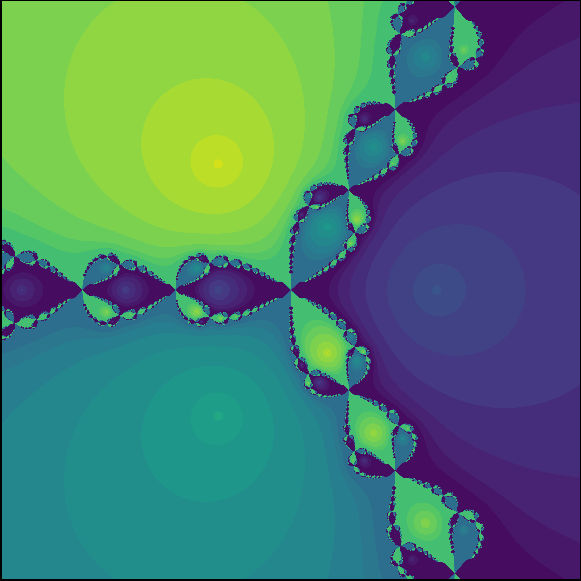
\includegraphics[
                width  = \paperwidth,
                height = \paperheight,
                keepaspectratio]{hires.png}
        }
    }
    \newgeometry{inner=0pt, outer=0pt}
    \begin{center}
        \noindent\fcolorbox{ThemeFrame}{ThemeBG}{
            \parbox{0.5\textwidth}{
                \begin{center}
                    \vspace{1em}
                    {\large\fontspec{Gill Sans}
                    \addfontfeature{LetterSpace=20.0}STEFFEN HAUG}\\[2em]
                    {\Huge\it Numerical Methods}
                    \vspace{1.618em}
                \end{center}
            }
        }
        \vfill
        {\ttfamily Assignment 2}
    \end{center}
\end{titlepage}

\begin{multicols}{2}


    \section*{Problem 1}
    The goal is to implement Newtons method for a generic function
    $\vec F: \R^2 \longrightarrow \R^2$.
    I will use a symbolic computation library to compute the
    Jacobian $\Jac[\vec F]$, which means the function needs to consist of
    {\ttfamily sympy}-compatible primitives.
    Except for this restriction, the functions can be generic.
    \begin{python}[
        caption={Helper functions for symbolic manipulation}
    ]
# file: src/alg.py
import numpy as np
from numpy import linalg as LA
import sympy as sp
import scipy.sparse as scsp


def symbolic_jac(py_fn):
    # Computes a symbolic jacobian matrix
    # for a function f : R^2 -> R^2.

    # compute the entries of the vector by
    # evaluating the function for sp-symbols
    x, y = sp.symbols('x y')
    f1, f2 = py_fn(x, y)
    F  = sp.Matrix([f1, f2])

    return F.jacobian([x, y])


def callable_fn(symbolic):
    # Create a function that substitutes
    # for the symbolic values.
    x, y = sp.symbols('x y')
    return sp.lambdify(
        [x, y], symbolic, 'numpy'
    )
    \end{python}
    Armed with some auxillary functions to handle the symbolic
    computation, we implement the iteration using
    the Newton method equation
    \[
        \vec x = \vec x - \Jac[\vec F]^{-1} \vec F(\vec x)
    \]
    \begin{python}[caption={Newton's method}]
# file: src/alg.py
MAX_ITER = 100

def solve(F, x0, tol=1E-6):
    x, y = x0

    J  = symbolic_jac(F)

    # singular jacobian means trouble
    Jfn = callable_fn(J)
    assert LA.det(Jfn(x, y)) != 0

    # function-version of the Jacobian
    Ji = callable_fn(J.inv())

    def step(f, Ji_f, x):
        # computes the next iteration using the
        # Newton method equation.
        # r is the previous step
        return x - Ji_f(*x).dot(f(*x))

    for _ in range(MAX_ITER):
        px, py = x, y
        x,  y  = step(F, Ji, (x, y))
        yield x, y

        # check the tolerance criteria
        if LA.norm(F(x, y)) < tol:
            break
        if LA.norm((x - px, y - py)) < tol:
            break

def last(it):
    # run an iterator to the end
    x = None
    for x in it: pass
    return x
    \end{python}
    \vspace{-0.5\baselineskip}
    \begin{python}[frame=b,numbers=none]
>>> from src.alg import solve, last
>>> def F(x, y):
...     return x**2 + y**2 - 2, x - y

>>> solve(F, (-1,0))
<generator...>
>>> last(solve(F, (-1,0)))
(-1.000000000013107, -1.000000000013107)
>>> last(solve(F, (1,0)))
(1.000000000013107, 1.000000000013107)
    \end{python}
    The interactive session shows how the function can be used,
    (it may not be so obvious since it is implemented
    as a generator-function, so we can collect the error {\em from outside};
    single resposibility principle and so on)
    and that it is correct at least for two points in different
    basins of attraction for the equation
    \[
        \vec F(x, y) = \begin{pmatrix}
            x^2 + y^2 - 2 \\
            x - y
        \end{pmatrix} \,\text,
    \]
    which has its true roots in $(-1, -1)$ and $(1, 1)$.

    \subsection*{Quadratic convergence}
    We want to verify that Newtons method converges quadratically,
    also in the multivariable case.
    To see this, we want to evaluate the limit
    \[
        \mu = \lim_{n \longrightarrow \infty}
            \frac{\Norm[2]{\vec x_{n+1} - \vec x_n}}
                 {\Norm[2]{\vec x_n - \vec x_{n-1}}^2}
        \,\text.
    \]
    Obviously, we don't have an infinite number of terms of $\Seq{\vec x_n}$.
    The best we can do is approximate $\mu$ by the ratios of our finite sequence.
    \begin{python}[
        caption={Computing the sequence of ratios}
    ]
approx = list(solve(F, (1000, 0), tol=1E-15))

def pairs(L):
    yield from zip(L[1:], L)

def diffs(L):
    for (xn, yn), (xm, ym) in pairs(L):
        yield (xn - xm, yn - ym)

def norms(vs):
        for v in vs: yield LA.norm(v)

norms_of_diffs = list(norms(diffs(approx)))

for p, q in pairs(norms_of_diffs):
    print(p/q**2)
    \end{python}
Which produces the following values.
Note that we need to use a very low tolerance,
otherwise we will not see anything resembling convergence at all.
    \begin{table}[H]
        \centering
        \caption{The sequence $\Seq{\mu_n}$ of ratios of error.}
        \begin{tabular}{c S[table-format=1.6]}
            \hline\hline
            \bfseries Iteration & $\mu_n$ \\
            \hline
            1  & 0.001414\\
            2  & 0.002828\\
            3  & 0.005656\\
            4  & 0.011309\\
            5  & 0.022596\\
            6  & 0.045009\\
            7  & 0.088582\\
            8  & 0.166701\\
            9  & 0.272763\\
            10 & 0.341980\\
            11 & 0.353357\\
            12 & 0.353553\\
            13 & 0.354073\\
            \hline
        \end{tabular}
    \end{table}\noindent
    It seems like the sequence settles on $\mu \approx 0.35$,
    which indicates quadratic convergence.
    \begin{figure}[H]
        \centering
        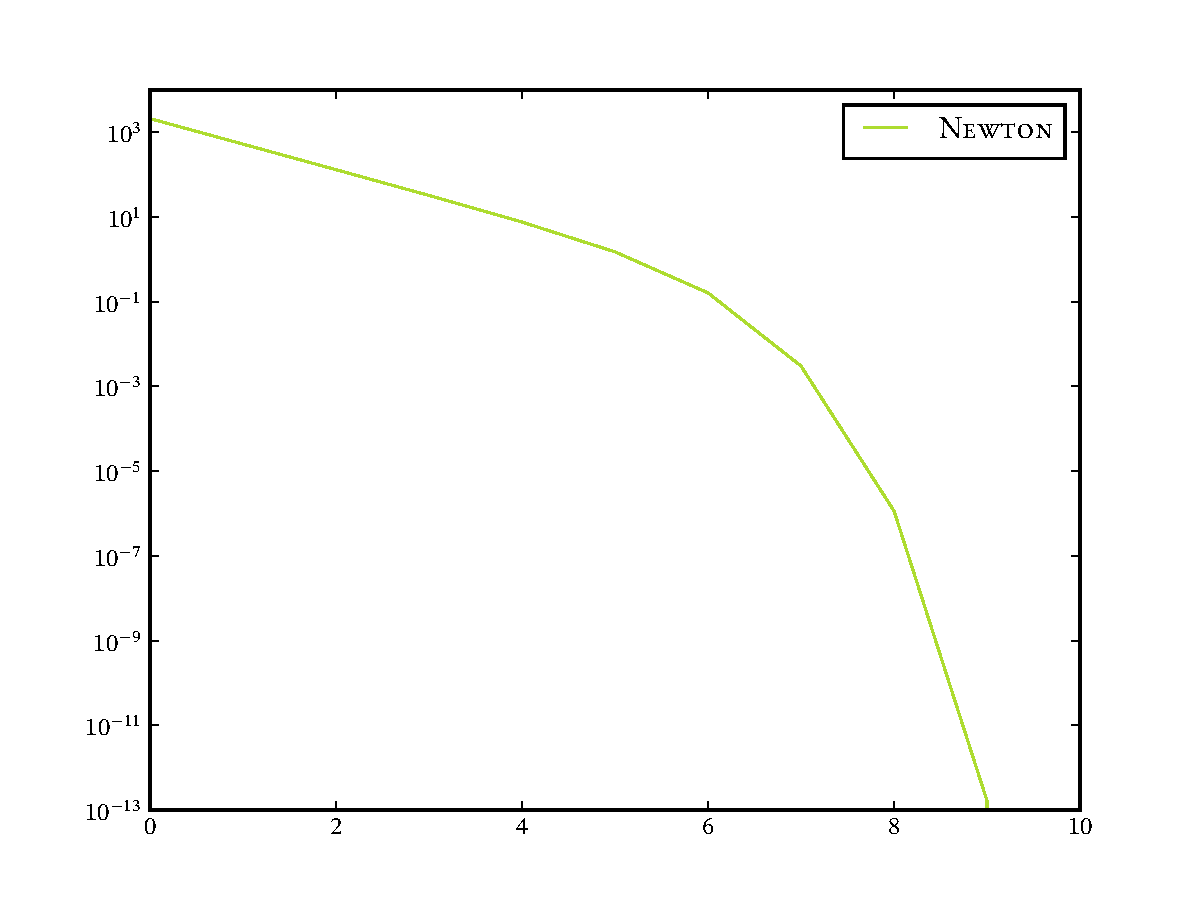
\includegraphics[width=0.75\columnwidth]{f_norms}
        \caption{
            Convergence of Newton's method with the norm $\Norm[2]{\vec F(x, y)}$
        }
        \label{fig:f_norms}
    \end{figure}\noindent

    \begin{figure}[H]
        \centering
        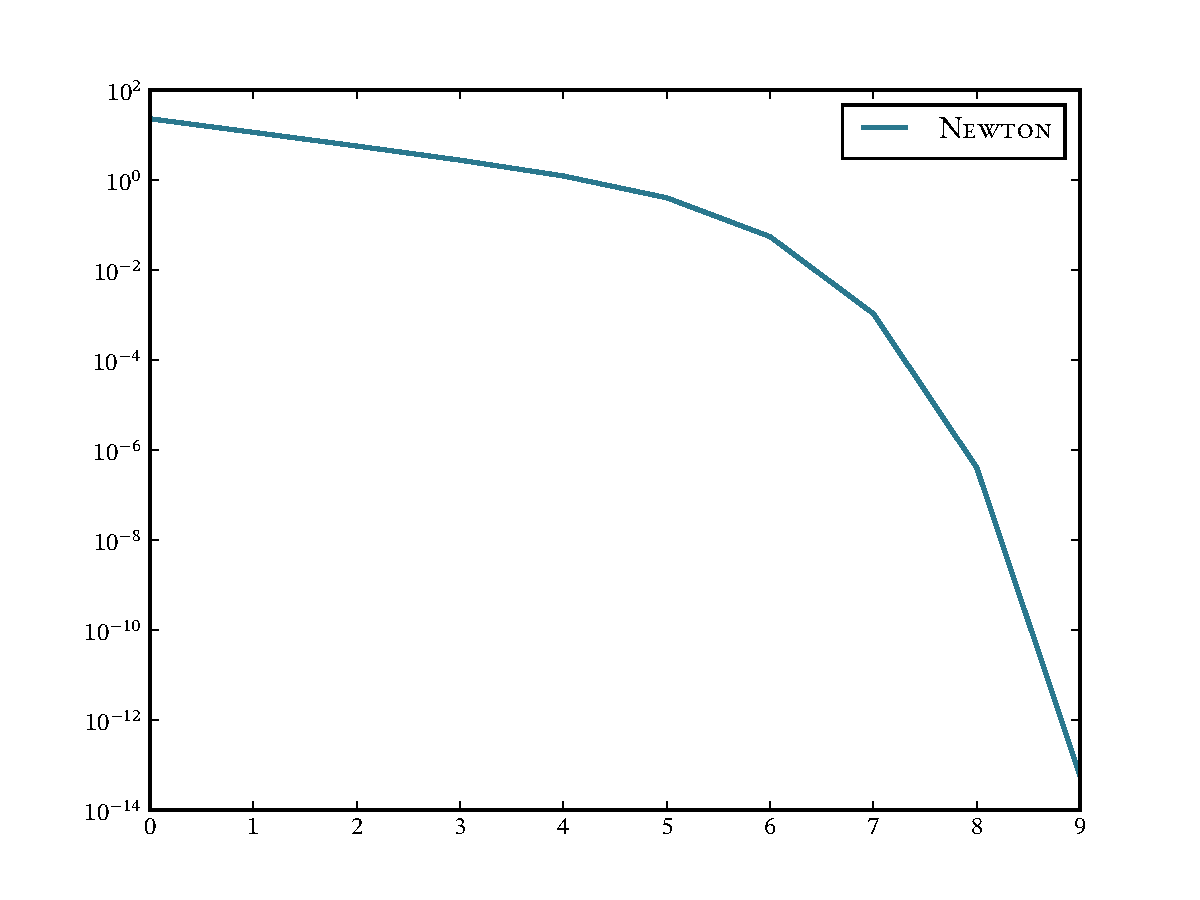
\includegraphics[width=0.75\columnwidth]{diff_norms}
        \caption{
            Convergence of Newton's method with the norm
            $\Norm[2]{\vec x_{k+1} - \vec x_k }$
        }
        \label{fig:diff_norms}
    \end{figure}\noindent
    The figures indicate that the convergence is at least superlinear.
    It is not easy to read from an image exacly how fast the convergence is,
    but with the estimated $\mu$, quadratic convergence seems likely.

    \subsection*{Convergence along diagonals}
    We want to see what happens as the method converges for
    two initial guesses that converges to different solutions.
    \begin{figure}[H]
        \centering
        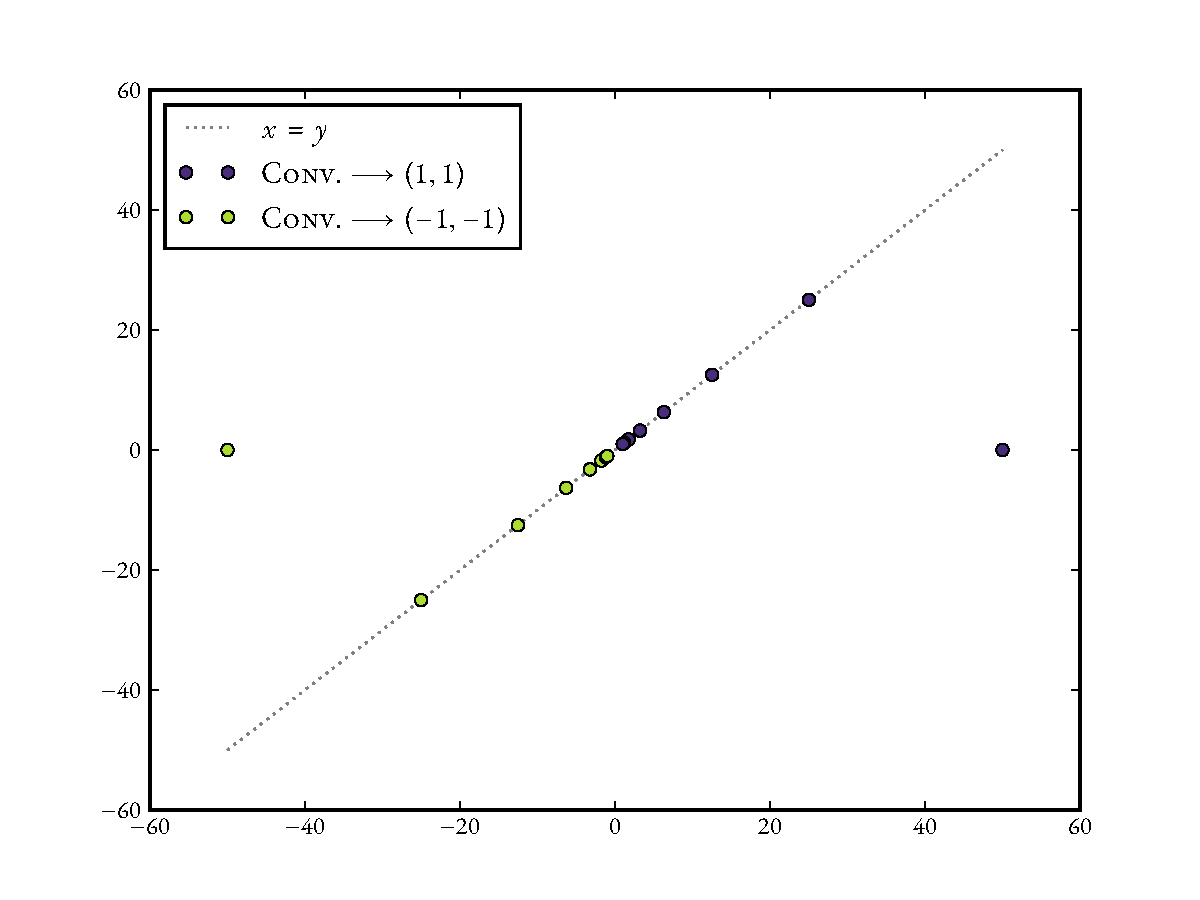
\includegraphics[width=0.75\columnwidth]{conv_pn}
        \caption{
            Convergence of Newton's method along the line $x = y$,
            starting at $\vec x = (-50, 0)$ and $\vec x = (50, 0)$.
        }
        \label{fig:conv_pn}
    \end{figure}\noindent
    As we can see, the solutions instantly ``jump'' to the
    $x = y$ diagonal, and converges along it.


    \section*{Optional problem}
    Given
    \[
        f(z) = z^3 - 1
    \]
    as a function $f: \C \longrightarrow \C$, we want to inspect the basins
    of attraction for Newton's mehod.
    We can view $f$ as a function $f: \R^2 \longrightarrow \R^2$ instead,
    and use the solver we already have.

    For every point in the complex plane, we are interested in which
    of the three roots Newton's method converges to.
    \begin{figure}[H]
        \centering
        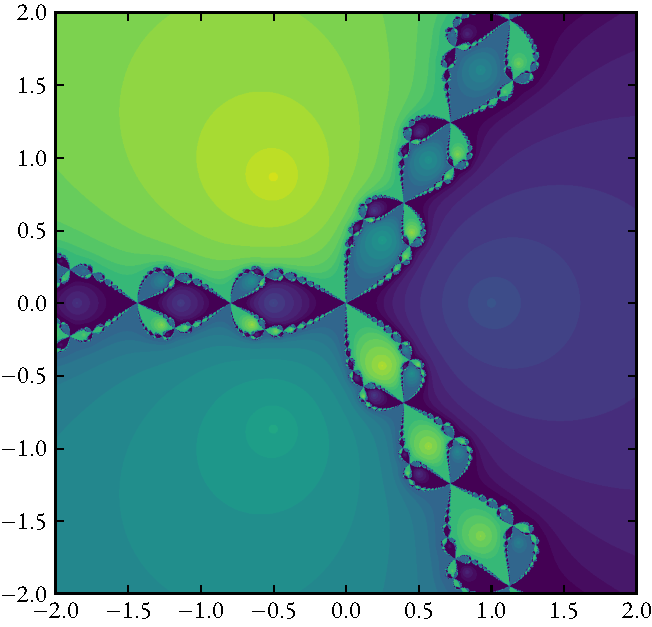
\includegraphics[width=0.75\columnwidth]{lores.pdf}
        \caption{
            Basins of attraction for Newton's method applied on
            $f(z) = z^3 - 1$.
        }
        \label{fig:basins}
    \end{figure}\noindent
    \Fig{basins} shows how the convergence forms three ``basins'' in
    a beautiful fractal pattern.


    \section*{Problem 2}
    We want to consider the linear system
    \[
        A \vec u = \vec f \,\text,
    \]
    where
    \[
        A = \left(
            L + (\Delta x)^2 k^2 I
        \right)
    \]
    is a matrix in $\R^{{n^2} \times\, {n^2}}$,
    and $\Delta x = 1/n$. Notice that $A$ is an operator
    that operates on vectors in $\R^{n^2}$, corresponding to
    an $n \times n$ lattice in a domain $\Omega$:

    \begin{figure}[H]
        \centering
        \includestandalone[width=0.9\columnwidth]{omega}
        \caption{
            Lattice points in $\Omega$.
        }
        \label{fig:omega}
    \end{figure}\noindent
    For any function $f(x, y)$ defined on $\Omega$, we can let
    \[
        \vec f = \begin{pmatrix}
            f_1 & f_2 & \cdots & f_l & \cdots & f_{n^2}
        \end{pmatrix}
        \,\text; \quad
        f_l = f(x_i, y_i) \,\text,
    \]
    where
    \[
        \left\{\begin{array}{l}
            x_i = i \cdot \Delta x \\
            y_j = j \cdot \Delta x \\
            l = \left(j - 1\right)n + i \\
        \end{array}\right.
    \]
    which corresponds exactly to ``sampling'' $f$ at the lattice points:
    $x_i = x_i(i)$ and $y_j = y_j(j)$ maps integer indeces $i$ and $j$
    to lattice points bijectively.
    $l = l(i,j)$ maps the same indeces to an index into a vector in $\R^{n^2}$
    bijectively.
    Thus, there is a bijective correspondance between lattice points
    and vector components.
    If we consider a concrete function
    \[
        f(x, y) \coloneqq \exp{\left(
            -50 \left(
                \left(x - \frac{1}{2}\right)
                + \left(y - \frac{1}{2}\right)
            \right)
        \right)}
    \]
    defined on $\Omega$, the sampled data looks something like
    \Fig{sample} for a relatively low choice of $n$.
    \begin{figure}[H]
        \centering
        \includestandalone[width=0.9\columnwidth]{plot_fxy}
        \caption{
            $f(x, y)$ sampled across the lattice in $\Omega$.
        }
        \label{fig:sample}
    \end{figure}\noindent
    This sampling can be done succinctly in python, using
    a generator function:
    \begin{python}[
        caption={Program to sample functions over lattices}
    ]
def lattice(n):
    for j in range(n):
        for i in range(n):
            yield i/(n - 1), j/(n - 1)

def sample(F, n):
    # samples F over a n x n lattice.
    return np.array(
        [F(x,y) for x, y in lattice(n)]
    )
    \end{python}
    {\tt sample(F, n)} produces exactly the vector $\vec f$,
    for a given function {\tt F}, sampled over a lattice
    in $\Omega$ with $\Delta x = 1/n$.

    To solve the system $A\vec u = \vec f$, we want to use
    fix-point iteration:
    \begin{align*}
        A \vec u &= \vec f \\
        (M - N) \vec u &= \vec f \\
        M \vec u &= N \vec u + \vec f \\
        \vec u &= M^{-1} (N \vec u + \vec f)
    \end{align*}
    in this equation, $M^{-1}N$ and $M^{-1}\vec f$ are constants.
    It is sensible (and more efficient) to compute them once up-front and give them
    names.
    This gives the more orderly iteration
    \[
        \vec u \leftarrow C\vec u + \vec g \,\text,
    \]
    which converges by the Banach fixed-point theorem if
    $\vec x \mapsto C\vec u + \vec g$ is a contraction,
    which is the case as long as
    \[
        0 < \rho(C) \coloneqq \smashoperator{
            \max_{\lambda \text{ eig. of } C}
        } \lambda < 1
        \text.
    \]
    In python, this can be implemented as follows
    \begin{python}[
        caption={N-dimensional solver.}
    ]
# src/alg.py
def spectral_radius(M):
    return np.max(np.abs(LA.eigvals(M)))

def solve_nd_fpi(M, N, f):
    # solves the linear system (M - N)u = b by
    # fix-point iteration u = inv(M)(Nu + b).

    Mi = LA.inv(M)
    C  = Mi.dot(N)
    g  = Mi.dot(f)

    assert spectral_radius(C) < 1

    u = g
    for _ in range(MAX_ITER):
        u = C.dot(u) + g
        yield u
    \end{python}
    provided we already have a choice of $M$ and $N$.
    Several ways to choose these matrices are possible,
    and we want to be able to choose.
    \begin{python}[
        caption={Argument-``parser'' and choice of $M$, $N$.}
    ]
# src/alg.py

def jacobi_mat(A):
    # Jacobi method
    M = np.diag(A.diagonal())
    N = M - A
    return M, N

def gs_mat(A):
    # Gauss-Seidel
    M = np.tril(A)
    N = M - A
    return M, N

def sor_mat(A, omega):
    # successive over-relaxation
    D = np.diag(A.diagonal())
    L = np.tril(A, k=-1)
    M = D + omega*L
    N = M - A
    return M, N

def choose_matrices(A, method="jacobi", omega=1.0):
    # pick a method based on the parameter
    # i have included some redundant parameters
    # so it is possible to write "shorthand"
    # upper-case also works.
    M, N = {
        # Jacobi method
        "jacobi":        jacobi_mat,
        "j":             jacobi_mat,
        # Gauss-Seidel method
        "gauss-seidel":  gs_mat,
        "gs":            gs_mat,
        # Successive over-relaxation
        "sor": lambda A: sor_mat(A, omega),
    }[method.lower()](A)

    return M, N


def solve_nd(A, f, method="jacobi", omega=1.0):
    # solve Ax = b.
    # returns an iterator over tuples (u, r),
    # where u is successively better solutions,
    # and r is the residual vector.
    # omega is unused unless "sor" is specified

    M, N = choose_matrices(A,
                           method=method,
                           omega=omega)

    for u in solve_nd_fpi(M, N, f, tol=tol):
        # compute the residual
        r = f - A.dot(u)
        yield u, r
    \end{python}
    Now, given some matrix $M$, and some vector $\vec b$,
    we can solve the system $M\vec u = \vec b$.
    Notice that, again, the system is implemented in such a way that it
    produces succesively better and better approximations.
    It also computes a residual vector which it gives us along with
    each approximation as a tuple {\tt (u, r)}.
    This makes the API a little clunky if all we want to do is
    compute the solution of some system, but it makes it easy to
    work with the data as a sequence.
    If all we want is the solution, we need the left-hand element of
    the last tuple.

    \subsection*{Testing the solver for a trivial problem}
    We want to make sure our code is correct for a simple problem,
    just so that we can have {\em some} confidence that it actually
    works.
    Solving a simple system, which we know has a solution,
    such as
    \[
        \arraycolsep=1.4pt\def\arraystretch{1}
        \left\{\begin{array}{rcrcr}
            3x &-&  y &=&  1 \\
            2x &+& 2y &=&  0 \\
        \end{array}\right.
    \]
    would give us a good hint about possible errors we might have made.
    (By insertion it is easy to verify that $x = 1/4$ and $y = -1/4$ is a solution)
    \begin{python}
# interactive session
>>> from src.alg import solve_nd, last
>>> import numpy as np

>>> A = np.array([[3, -1],
...               [2,  2]])

>>> b = np.array([1, 0])

>>> u, v = last(solve_nd(A, b, method="Jacobi"))
>>> u
array([ 0.25, -0.25])

>>> u, v = last(solve_nd(A, b, method="GS"))
>>> u
array([ 0.25, -0.25])

>>> u, v = last(solve_nd(A, b, method="SOR"))
>>> u
array([ 0.25, -0.25])
    \end{python}
    As we can see, all the methods give the correct solution.

    \subsection*{Solving the original problem}

    We can find a solution to our original problem,
    fixing $n = 10$ and $k = 1/100$, by setting up
    \begin{python}
from src.alg import solve_nd, sample
from asc.alg import A as gen_A
import numpy as np

n = 10
k = 1/100

def F(x,y):
    return np.exp(
        -50 * ((x - 1/2)**2 + (y - 1/2)**2)
    )

f = sample(F, n)
A = gen_A(k, n)
    \end{python}
    Here, {\tt src.alg.A} is an algorithm provided for us that generates $A$.
    {\tt f} is the vector obtained when sampling
    \mbox{{\tt F} $\coloneqq f(x, y)$} across the lattice defined by $n = 10$.
    The {\tt sample}-function is the same one we developed earlier.

    Given these structures, we are interested in comparing the performance of each of
    the three methods when solving the system $A \vec u = \vec f$.

    \subsection{Comparing the convergence}
    We are interested in looking at the relative residual
    $\Norm[2]{r_n} / \Norm[2]{r_0}$ for each iteration $n$ of the
    algorithms. These can be computed with the following Python-program:
    \begin{python}
def right(it):
    for _, x in it: yield x

def relative_residual(appr):
    # we need a list, because
    # we can't peek iterators
    assert type(appr) == list
    a = LA.norm(appr[0][1])
    for r in right(iter(appr)):
        yield LA.norm(r) / a
    \end{python}
    \Fig{residuals} shows the relative residuals for each of the methods,
    including three different values for $\omega$ in the case of
    successive over-relaxation.
    \begin{figure}[H]
        \centering
        \includestandalone[width=0.9\columnwidth]{residual}
        \caption{
            The residuals of each method for a given iteration.
        }
        \label{fig:residuals}
    \end{figure}\noindent




    \subsection{Comparing the relative time}
    \subsection{Spectral radius and convergence}
    Considering \Fig{residuals},
    it is quite clear that after a certain number of iterations,
    the convergence is linear.
    In hindsight, this is not so surprising.
    Consider $\vec u$ as a linear combination of an eigen-basis
    $\beta = \Seq{v_i}$
    given by the eigenvectors of $C$.
    Then the operation of $C$ on
    \[
        \vec u = \sum_i a_i \cdot v_i
    \]
    is to scale each component of $\vec u$ by the corresponding eigenvalue:
    \begin{align*}
        C \vec u &= \sum_i \lambda_i \cdot a_i \cdot v_i \\
        \implies C^n \vec u &= \sum_i \lambda_i^n \cdot a_i \cdot v_i
        \text.
    \end{align*}
    Since $0 < \rho(C) < 1$, each component converges by itself,
    so the sequence converges in its entirety, but
    {\em only as fast as the slowest component converges!}
    Naturally, the slowest converging component converges linearly,
    with $\mu = \rho(C)$.

    Using Python, we can easily compute the spectral radiuses
    of the iteration matrices.
    \begin{table}[H]
        \centering
        \caption{The spectral radiuses of the iteration matrices for each method}
        \begin{tabular}{c S[table-format=1.6]}
            \hline\hline
            \bfseries Algorithm & \bfseries Spectral Radius \\
            \hline
            Jacobi                      & 3.999999\\
            Gauss-Seidel                & 3.999999\\
            S. O. R. $(\omega = 0.25)$  & 3.999999\\
            S. O. R. $(\omega = 0.50)$  & 3.999999\\
            S. O. R. $(\omega = 0.75)$  & 3.999999\\
            \hline
        \end{tabular}
        \label{table:rhos}
    \end{table}\noindent
    \Tab{rhos} reveals that they all have the same asymptotic rate of convergence.


    \subsection{Relation between $k$, $\Delta x$ and convergence}


\end{multicols}
\end{document}
